\chapter{Deep Learning}
%\addcontentsline{toc}{chapter}{4. Classification/Deep Learning Methods}
\hl{not sure how much of a summary to give here. Maybe skip is because I go into detail below?}
Schaefer \etal \cite{schaefer_name_2011} were able to use the unique time course of the component responsible for the most variance to differentiate between stimuli.
Analyzing our components we have not yet been able to reproduce this significant stimulus classification accuracy. 
%This could be caused by our much smaller number of trials which are substantially longer than those used by \cite{schaefer_name_2011}. 
%On average we used \hl{X number of} trials in our analysis, while Schaefer et al. (2011) collected 145 trials of each of their stimuli.
 
We approached our data using a technique from the computer science field of Deep Learning called a convolutional neural network (\ac{CNN}) in order to classify our data.
A \ac{CNN} contains one or more convolutional layers that process the data.
In these layers the input is processed by a filter (weight matrix) that is trained using back propagation. 
These filters move along the input dimensions with a constant step size and at each position an output value is computed.
Our \ac{CNN} was optimized for this classification task and includes three processing layers.
%The first layer consists of a filter of electrode weights that reduces the 64 channel data to a single data stream and gives us information about which EEG channels are important for differentiating classes.
%The second layer consists of an optimized filter that convolves the single data stream.
%This results in a compressed representation of the original EEG data.
%In the third layer, these compressed representations are classified by comparing them to learned temporal patterns (one for each class)
%During the training phase these compressed representations of each of our stimuli are optimized using back propagation.
%During the testing phase the compressed representations describing the test data are compared to the optimized versions. 
%This matching in the third layer is what allows us to classify our data.
The full explanation of how we arrived at the best model can be found in (cite paper) \hl{include as appendix?}.

\section{Layer 1: Similarity Constraint Encoding}
The first layer was pre-trained and then was not changed during training of the entire model. 
432 trials (9 subjects x 12 stimuli x 4 trials) were used for training. 
The third trial from each subject's data was left out to be used as the test set for later model testing (108 trials (9 subjects x 12 stimuli x 1 trial) ).
%Techniques such as \ac{PCA} and \ac{ICA} can be used to find stable and representative patterns (or components) in the \ac{EEG} data.
%Another way to learn such patterns is by using \acp{CAE}.
%\acp{CAE} are a special variant of \acp{CNN} that encode their input using convolution into a compressed internal representation which is then decoded using de-convolution into the original space trying to minimize the reconstruction error. 
%Using \acp{CAE} allows us to learn individually adapted components that are linked between subjects.
We wanted to find features in the data that are not only stable across trials and subjects, but also allow us to distinguish between classes. 
In order to identify such features we used a pre-training strategy called \emph{similarity-constraint encoding}.
% in which the \ac{CAE} is trained to encode relative similarity constraints. 
As introduced by \cite{schultz_learning_2004}, a relative similarity constraint $(a,b,c)$ describes a relative comparison of the trials $a$, $b$ and $c$ in the form ``$a$ is more similar to $b$ than $a$ is to $c$.''
Here, $a$ is the reference trial for the comparison.
This similarity constraint is used as a cost function for learning features. 
The number of violated constraints is minimized using the standard back propagation training technique used for artificial neural networks.
To this end, we combine all pairs of trials $(a,b)$ from the same class %(as described in \autoref{sec:CTE}) 
with all trials $c$ from other classes demanding that $a$ and $b$ are more similar.
The topographic representation of the features learned by this \ac{SCE} is visualized in Layer 1 of \autoref{fig:model_W}. 
The coloured areas represent the regions that are most important for \emph{differentiating} classes. 
These features act as electrode weights.
As this filter processes the raw data 64 channels are reduced to a single data stream. 
\begin{figure}[h] 
  \begin{center}
    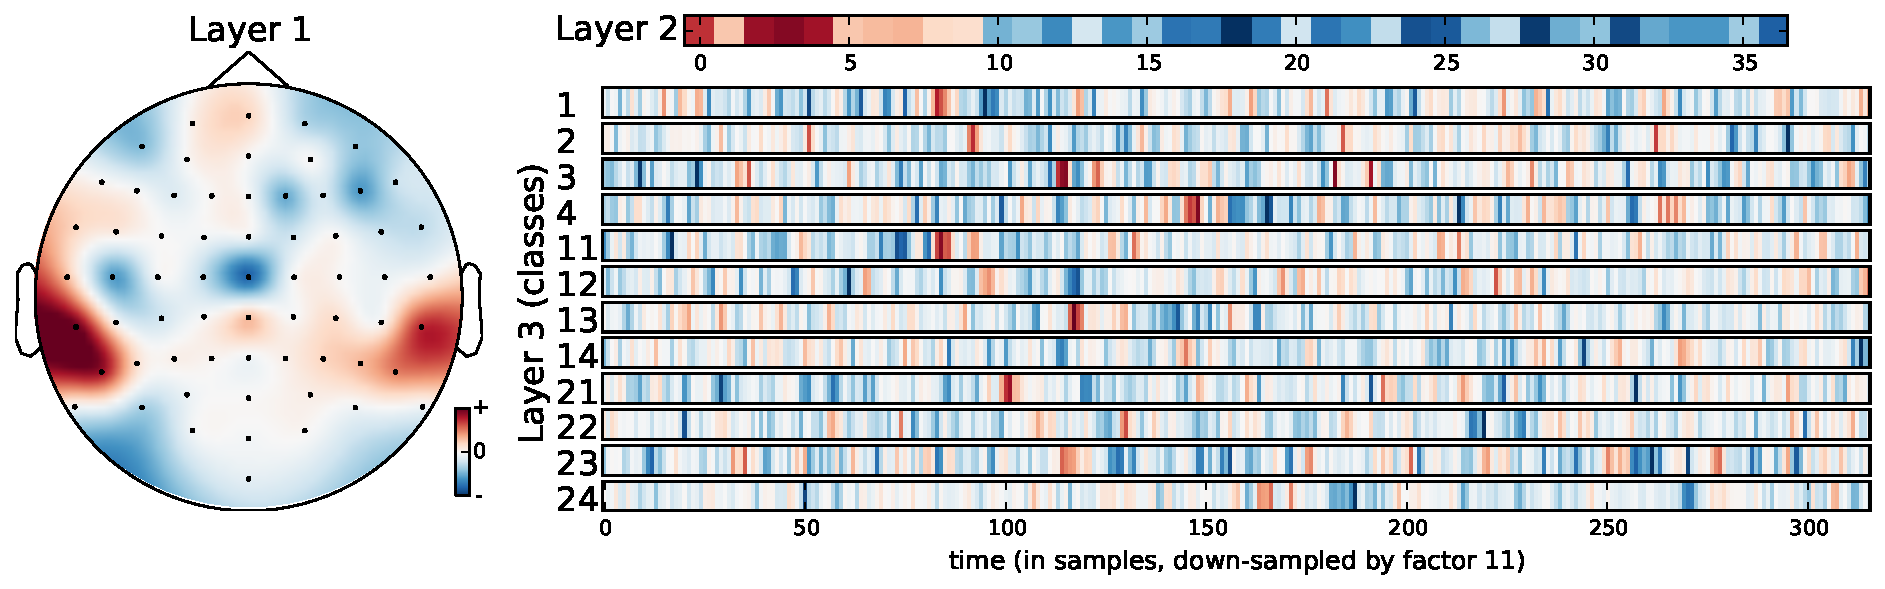
\includegraphics[width=\textwidth,keepaspectratio=true]{Figures/model_W}
%   \\\vspace{-0.8em}
    \caption{Visualization of \ac{CNN}, which processes raw EEG at a sampling rate of 512\,Hz.
    Layer 1 was pre-trained using similarity-constraint encoding.}
    \label{fig:model_W}
  \end{center}
%  \vspace{-1em}
\end{figure}
\section{Layer 2: Convolution Filter \& Layer 3: Templates}
Layers two and three were trained together with supervised learning and optimized by back propagation through the entire model with a cost function to minimize classification error.
We employed a 9-fold cross validation scheme by training on the data from 9 subjects (384 trials) and validating on the remaining subject (48 trials).
The cross-validation was done within the training set with the aim of finding the optimal hyper-parameters (learning rate, filter size, etc.) for our neural network. 
The final version of layer 2 and 3 is an average of the model parameters over all 9 fold models (see Layer 2 in \autoref{fig:model_W}).
\section{How the whole thing works (title)}
The single data stream output from layer 1 enters the second layer where it is convolved with a filter. 
After the data is convolved with the filter in layer 2 and then pooled with a subsampling factor of 11 a single stream of data, which is an optimized, compressed representation of the original raw EEG data, is produced.
These representations are shown in Layer 3 of \autoref{fig:model_W}. 

The model was then tested with the test set of 108 trials. 
The test data passes through the layers of the model and the representations produced in layer 3 are compared against the optimized versions. 
The dot product of the test data's output from layer 2 is taken with each of the optimized layer 3 representations created during the training phase. 
This produces 12 values (one for each stimulus) that describe the similarity of the test data with each of the optimized layer 3 representations. 
The test data is given the label of the stimulus whose representation it matches the most, i.e. the highest similarity value from the dot product. 